\include{template}
%\cfoot{} %% if no page number is needed

\begin{document}

\begin{header}
Outils mathématiques
\end{header}

\section*{Le produit en croix}

Prenons l'exemple de la masse volumique \og rho \fg{} notée $\rho$ (en $\mathrm{kg/m^3}$) exprimée en fonction de la masse $m$ ($\mathrm{kg}$) et du volume $V$ ($\mathrm{m^3}$).
On sait que :
\begin{equation}
\rho = \frac{m}{V}.
\nonumber
\end{equation}

Dans un exercice ou en TP, on vous demande de trouver $m$.
Comment faire ?


\subsection*{Le triangle}

\begin{conseil}
Je commence par dessiner le triangle avec un T dedans.
La barre horizontale du T symbolise une division, la verticale une multiplication.
Pour remplir le triangle, je commence par la case du haut, celle au dessus de la barre horizontale comme dans l'équation : on y met la masse $m$.
Le volume $V$ est en bas à droite dans l'équation, je le met aussi en bas à droite dans le triangle.
Reste la masse volumique $\rho$ que je met dans la case vide restante, en bas à gauche.
\end{conseil}

\begin{figure}[h]
\center
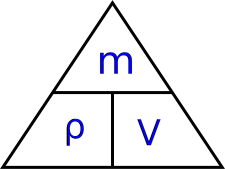
\includegraphics[scale=0.5]{images/pyramide_fraction.png}
\end{figure}

\begin{conseil}
Pour trouver $m$, je cache le haut de la pyramide.
Il ne reste que $\rho$ et $V$ séparés par une barre verticale : je dois les multiplier.
On a donc
\begin{equation}
m = \rho \times V
\nonumber
\end{equation}
\end{conseil}

\subsection*{Substitution}

\begin{conseil}
Je trouve une équation simple avec des chiffres, qui a la même forme que l'équation de la masse volumique.
Par exemple :
\begin{equation}
5 = \frac{10}{2}.
\nonumber
\end{equation}
Le 5 occupe la place du $\rho$, le 10 celle du $m$ et le 2 celle de $V$.

Pour retrouver $m$, j'écris 10 = ? en fonction de 5 et 2.
On est obligé d'écrire :
\begin{equation}
10 = 5 \times 2,
\nonumber
\end{equation}
et donc en remplaçant à nouveau par les lettres, on retrouve
\begin{equation}
m = \rho \times V.
\nonumber
\end{equation}
\end{conseil}

\section*{Conversions (1)}

Les préfixes permettent d'alléger l'écriture des résultats.

\begin{table}[h]
\center
\begin{tabular}{l|c|c|c|c|c|c|c}
préfixe         & kilo & hecto& déca & ...  & déci & centi& milli\\
abréviation     & k... & h... & da...& ...  & d... & c... & m... \\
facteur         & 1000 & 100  & 10   & 1    & 0{,}1& 0{,}01& 0{,}001 \\
puissance de 10 &$10^3$&$10^2$&$10^1$&$10^0$&$10^{-1}$&$10^{-2}$&$10^{-3}$ 
\end{tabular}
\end{table}

\section*{Conversions (2)}

\begin{conseil}
Pour les volumes, il faut surtout se rappeler que \unit{1}{L} = \unit{1}{\deci\meter^3}.
\end{conseil}


\end{document}